\documentclass[letterpaper,pdftex]{article}

\setlength{\textwidth}{168mm}
\setlength{\textheight}{210mm}
\setlength{\oddsidemargin}{0cm}
\setlength{\topmargin}{0cm}
\setlength{\headheight}{48pt}
\addtolength{\textheight}{-25pt}
\voffset -0.5in

\usepackage{natbib}
\usepackage[utf8]{inputenc}
\usepackage[spanish]{babel}
\usepackage{xcolor,graphicx}
\graphicspath{{Figures/}}
\usepackage{fancyhdr}
\usepackage{multirow}
\usepackage{siunitx}
\usepackage{hyperref}
\hypersetup{
    colorlinks,
    citecolor=blue,
    filecolor=black,
    linkcolor=blue,
    urlcolor=black
}
\usepackage{epstopdf}
%To code editing
\usepackage{listings}
\usepackage{xcolor}
\definecolor{codegreen}{rgb}{0,0.6,0}
\definecolor{codegray}{rgb}{0.5,0.5,0.5}
\definecolor{codepurple}{rgb}{0.58,0,0.82}
\definecolor{backcolour}{rgb}{0.95,0.95,0.92}

\lstdefinestyle{mystyle}{
    backgroundcolor=\color{backcolour},   
    commentstyle=\color{codegreen},
    keywordstyle=\color{magenta},
    numberstyle=\tiny\color{codegray},
    stringstyle=\color{codepurple},
    basicstyle=\ttfamily\footnotesize,
    breakatwhitespace=false,         
    breaklines=true,                 
    captionpos=b,                    
    keepspaces=true,                 
    numbers=left,                    
    numbersep=5pt,                  
    showspaces=false,                
    showstringspaces=false,
    showtabs=false,                  
    tabsize=2
}

\lstset{style=mystyle}

% -------------URL style
\hypersetup{
    colorlinks=true,
    linkcolor=blue,
    filecolor=magenta,      
    urlcolor=cyan,
    pdftitle={Overleaf Example},
    pdfpagemode=FullScreen,
    }

\urlstyle{same}
% --------------

%\usepackage[autolinebreaks,useliterate]{mcode}
\pagestyle{fancy}
\renewcommand{\headrule}{\color{gray}
\hrule width\headwidth height\headrulewidth \vskip-\headrulewidth}
\renewcommand{\footrule}{{\color{gray}
\vskip-\footruleskip\vskip-\footrulewidth
\hrule width\headwidth height\footrulewidth\vskip\footruleskip}}
\renewcommand{\headrulewidth}{1.5pt}
\renewcommand{\footrulewidth}{1.5pt}

\usepackage{caption}
\usepackage{subcaption}

%----Maths
\usepackage{amsmath}

\spanishdecimal{.}

\begin{document}
\fancyhead{}
\fancyfoot{}
\fancyhead[L]{
\begin{minipage}{3.5cm}
\begin{center}
	
\includegraphics[width=0.95\textwidth]{logousb.png}
\end{center}
\end{minipage}
\begin{minipage}{12cm}
\begin{flushleft}
\small \textsc{Universidad de San Buenaventura}\\
\small \textsc{Faculty of Engineeering}\\
\small \textsc{School of Mechatronics Engineering\\}
\end{flushleft}
\end{minipage}
}
\fancyhead[R]{
\begin{minipage}{3.0cm}
\begin{flushright}
\small \textsc{Foundations of Robotics}\\
\small \textsc{2021-II}
\end{flushright}
\end{minipage}
}
\fancyfoot[R]{\large \textbf{\thepage}}

\begin{minipage}{0.3\textwidth}
\begin{flushleft}
\textbf{Author:}\\
\textit{Nikolay Prieto Ph.D(c)}\\
\end{flushleft}
\end{minipage}
\begin{minipage}{0.7cm}
\textcolor{gray}{\rule{0.3cm}{2.5cm}}
\end{minipage}
\begin{minipage}{0.64\textwidth}
\Large{\textbf{Middle Term Workshop\\ DH \--- IK \--- FK \--- DK}}
\end{minipage}\\

\noindent
\textcolor{gray}{\rule{\textwidth}{0.5pt}}\\
\renewcommand{\tablename}{Tabla}
\renewcommand{\arraystretch}{1.2}
\renewcommand\contentsname{Contents}
\tableofcontents

\noindent
\textcolor{gray}{\rule{\textwidth}{0.5pt}}\\

\section{Objectives}
\begin{itemize}
\item To evaluate the concepts learnt so far in Industrial manipulators.
\end{itemize}

\section{Instructions}
\begin{itemize}
\item This assignment is individual.
\item Duration: 180 minutes.
\item You might validate your results with the computational resources: Sympy, rtb, etc.
\end{itemize}

\section{Question 1}


The \href{https://robots.ieee.org/robots/hrp4c/}{HRP-4C} robot is a humanoid robot with female features. The figure \ref{fig:HRP} shows the bottom of this robot, with six degrees of freedom. Units shown are in millimeters. It is desired to model the right leg of this robot using the Denavit-Hartenberg (DH) convention standard. The base system {0} is shown in the figure and is at hip level. The end system {6} to be used as the “end effector” is also shown in the figure \ref{fig:HRP}

\begin{figure}[h]
\centering
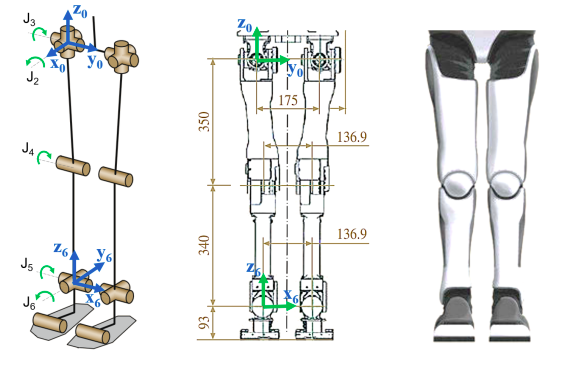
\includegraphics[scale=0.7]{HRP-4C.png}
\caption{General measures of the HRP-4C}\label{fig:HRP}
\end{figure}



Do the following

\begin{itemize}
\item Assign the missing reference frames to the right leg of the robot according to the convention Standard DH. The order of the joints is displayed as $J_i$, along with the direction of rotation. To facilitate the task, it is not necessary to indicate the y-axes. Note that the knee has some lateral displacement with regarding the waist.
\item Determine the table with the DH parameters that describe this robot.
\end{itemize}

\section{Question 2}

The kinematic model of an RPR robot with three degrees of freedom is described by Denavit-Hartenberg parameters shown in the following table, where $l_2 = 0.7$m

% Preview source code for paragraph 0

\begin{table}
\begin{centering}
\begin{tabular}{|c|c|c|c|c|}
\hline 
link & $d_{i}$ & $\theta_{i}$ & $a_{i}$ & $\alpha_{i}$\tabularnewline
\hline 
\hline 
1 & 0 & $q_{1}$ & 0 & 0\tabularnewline
\hline 
2 & $q_{2}$ & $-\frac{\pi}{2}$ & 0 & $\frac{\pi}{2}$\tabularnewline
\hline 
3 & 0 & $q_{3}$ & $l_{2}$ & $\frac{\pi}{2}$\tabularnewline
\hline 
\end{tabular}
\par\end{centering}
\caption{DH configuration for the RPR robot}

\end{table}

\begin{itemize}
\item Find the linear velocity and the angular velocity of the end effector of this robot, when having joint configuration $q=[\frac{\pi}{4}, 0.5, \pi]$, the joints have a change ration with respect to at the time of $q = (0.4, 0.1, 0.4)$. Units are in rad, m, rad/s, m/s, as appropriate.
\item Determine all the unique configurations of this robot, considering only the
part corresponding to position, it means, at linear speed.
\item The robot, with a quaternion configuration $q=[\frac{\pi}{4}, 0.5, \pi]$, is in contact with a table. It is desired the robot \--- maintaining this configuration \--- exerts a force (0.5, 0.5, 0.5) and a null moment on the table. Determine, if possible, the torques that should be applied to each motor to satisfy this restriction.
\item The orientation of the end effector of this robot is represented using a quaternion. The relationship between the change rate of a quaternion and the angular velocity is given by:

\begin{equation}
\omega=2\left[\begin{array}{cccc}
-\epsilon_{x} & w & -\epsilon_{z} & \epsilon_{y}\\
-\epsilon_{y} & \epsilon_{z} & w & -\epsilon_{x}\\
-\epsilon_{z} & -\epsilon_{y} & \epsilon_{x} & w
\end{array}\right]\dot{Q}
\end{equation}

Express the analitic Jacobian (you have not seen this, study for yourself.)



\end{itemize}


\bibliographystyle{plain}
\bibliography{biblio.bib}
\end{document}